\documentclass[final]{beamer}
\linespread{1.25}
\usepackage[T1]{fontenc}
\usepackage{lmodern}  
\usepackage{blindtext}
\usepackage[english]{babel} 
\usepackage{lipsum}
\usepackage[orientation=portrait,size=a0,scale=1.0]{beamerposter}
\usetheme{gemini}
\usecolortheme{nott}
\usepackage{graphicx}
\usepackage{booktabs}
\usepackage{tikz}
\usepackage{pgfplots}
\pgfplotsset{compat=1.14}
\usepackage{anyfontsize}
\usepackage{xcolor}
\usepackage[skip=2pt,font=normalsize]{subcaption}
\usepackage{adjustbox}
\usepackage{tikz}
\usetikzlibrary{shapes.geometric, arrows}
\tikzstyle{startstop} = [rectangle, rounded corners, minimum width=3cm, minimum height=1cm, text centered, text width = 10cm, draw=black, fill=white]
\tikzstyle{process} = [rectangle, minimum width=3cm, minimum height=1cm, text centered, text width = 6cm, draw=black, fill=white, text width = 10cm]
\tikzstyle{arrow} = [ultra thick,->,>=stealth]
\newlength{\sepwidth}
\newlength{\colwidth}
\setlength{\sepwidth}{0.025\paperwidth}
\setlength{\colwidth}{0.45\paperwidth}
\newcommand{\separatorcolumn}{\begin{column}{\sepwidth}\end{column}}

\title{Poster Title  Poster Title Poster Title Poster Title Poster Title Poster Title Poster Title Poster Title}
\title{ Illuminating the Practices of Internet Service Providers
}

\author{Jaanhvi Agarwal \and Amanda Anowi \and  Aaron Gember Jacobson}
\setbeamerfont{author}{size=\VeryLarge}
\institute[shortinst]{Department of Computer Science, Colgate University}
\setbeamerfont{institute}{size=\VeryHuge}

\logoleft{
\includegraphics[height=10cm]{Colgate_logo.png}}

\usepackage{pgf}

\begin{document}
\fontsize{33pt}{50pt}\selectfont

\begin{frame}[t]
\begin{columns}[t]
\separatorcolumn

\begin{column}{\colwidth}

\begin{block}{Goals}
Networks utilize routers to facilitate the transfer of data packets to and from the network. Due to the growing concern about energy usage in large-scale networks, our goal is to determine if it's feasible to estimate the power consumption of any given internet service provider (ISP). The difficulty in this is that ISPs do not release topology details and network vendors do not release power consumption information due to privacy reasons. Thus, we explore other means of obtaining this information without relying on ground truth data from ISPs or vendors.
\end{block}

  
\begin{exampleblock}{Research Questions}
\begin{enumerate}
    \item How can we count the number of routers are deployed in a network?
    \item How can we extract hardware information from these routers?
    \item How can we compute power consumption given hardware information?
\end{enumerate}
\end{exampleblock}

\begin{block}{Counting Routers}
We compared commonly-used network topology inferences from the Cooperative Association for Internet Data Analysis (CAIDA) with ground truth data we gathered using Internet2's router proxy. We found that the CAIDA dataset had extra routers and missing links. Further research is needed to identify potential factors contributing to these discrepancies.



\begin{figure}[h]
    \centering
    \begin{minipage}{0.6\textwidth}
        \centering
        \begin{adjustbox}{frame, bgcolor=black, center}
            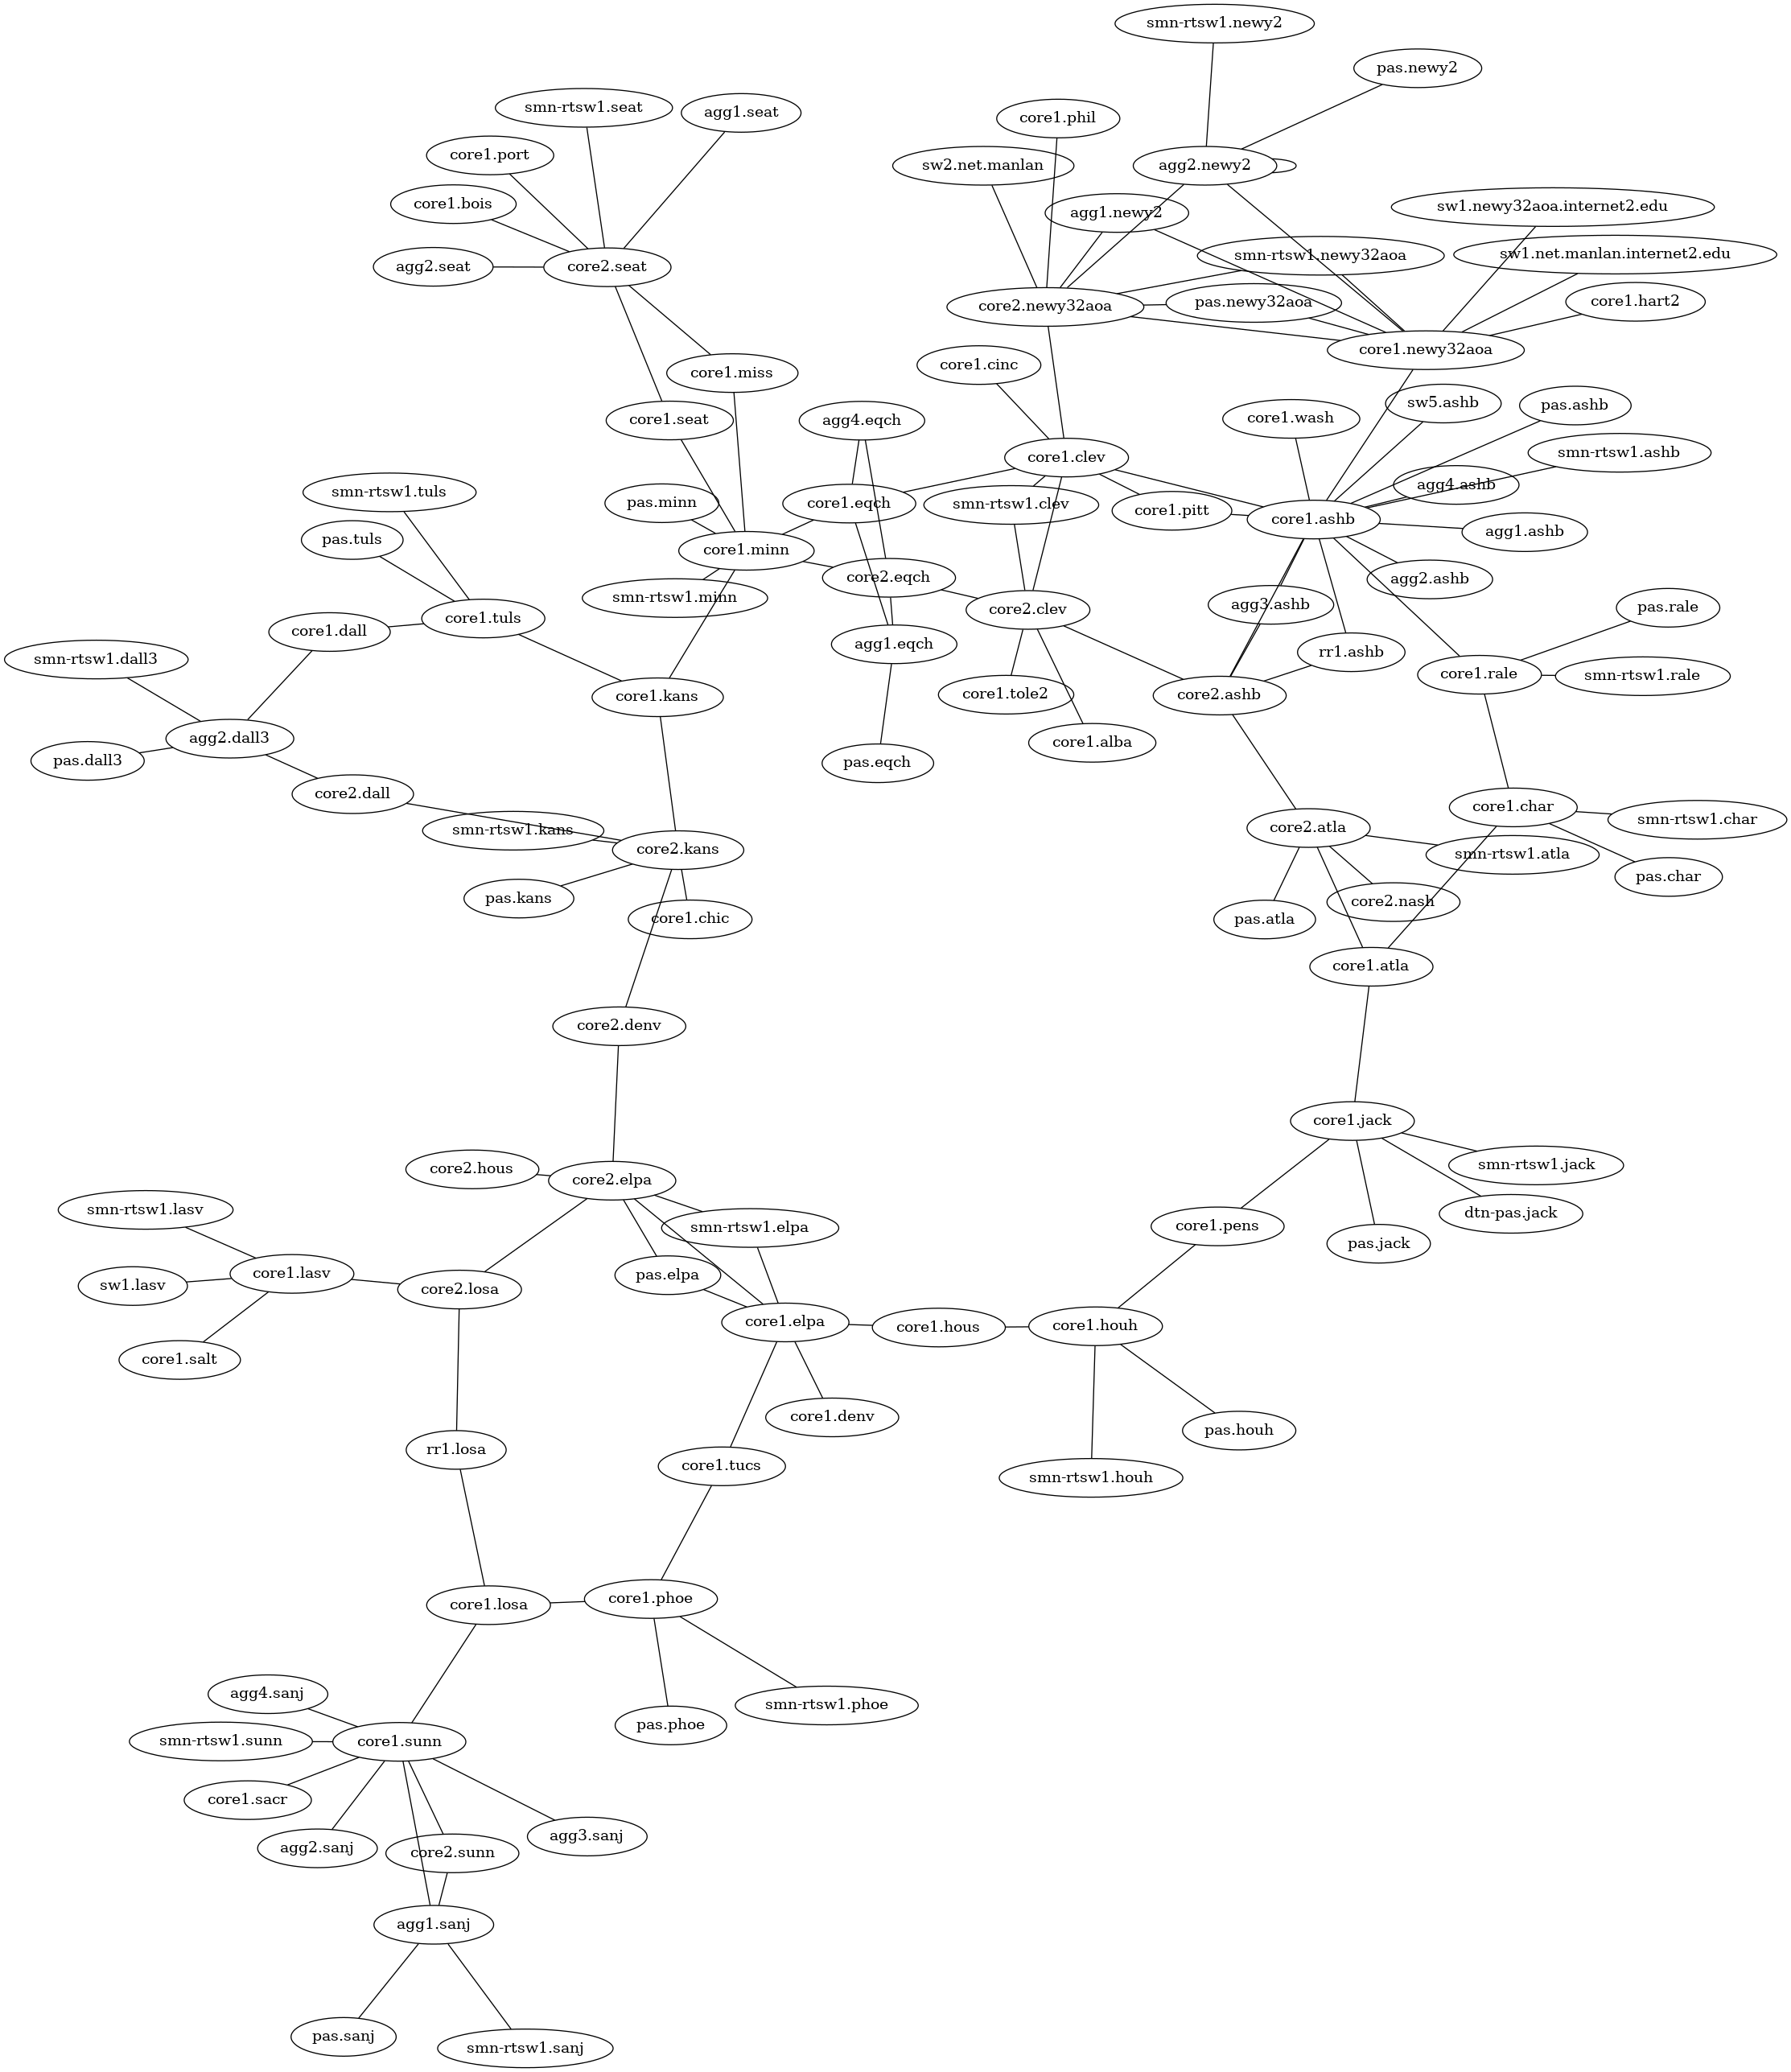
\includegraphics[width=\linewidth]{images/lldp_graph.png}
        \end{adjustbox}
        % \caption{Caption for image 1}
        \label{fig:image1}
    \end{minipage}
    \hfill
    \begin{minipage}{0.6\textwidth}
        \centering
        \begin{adjustbox}{frame, bgcolor=black, center}
            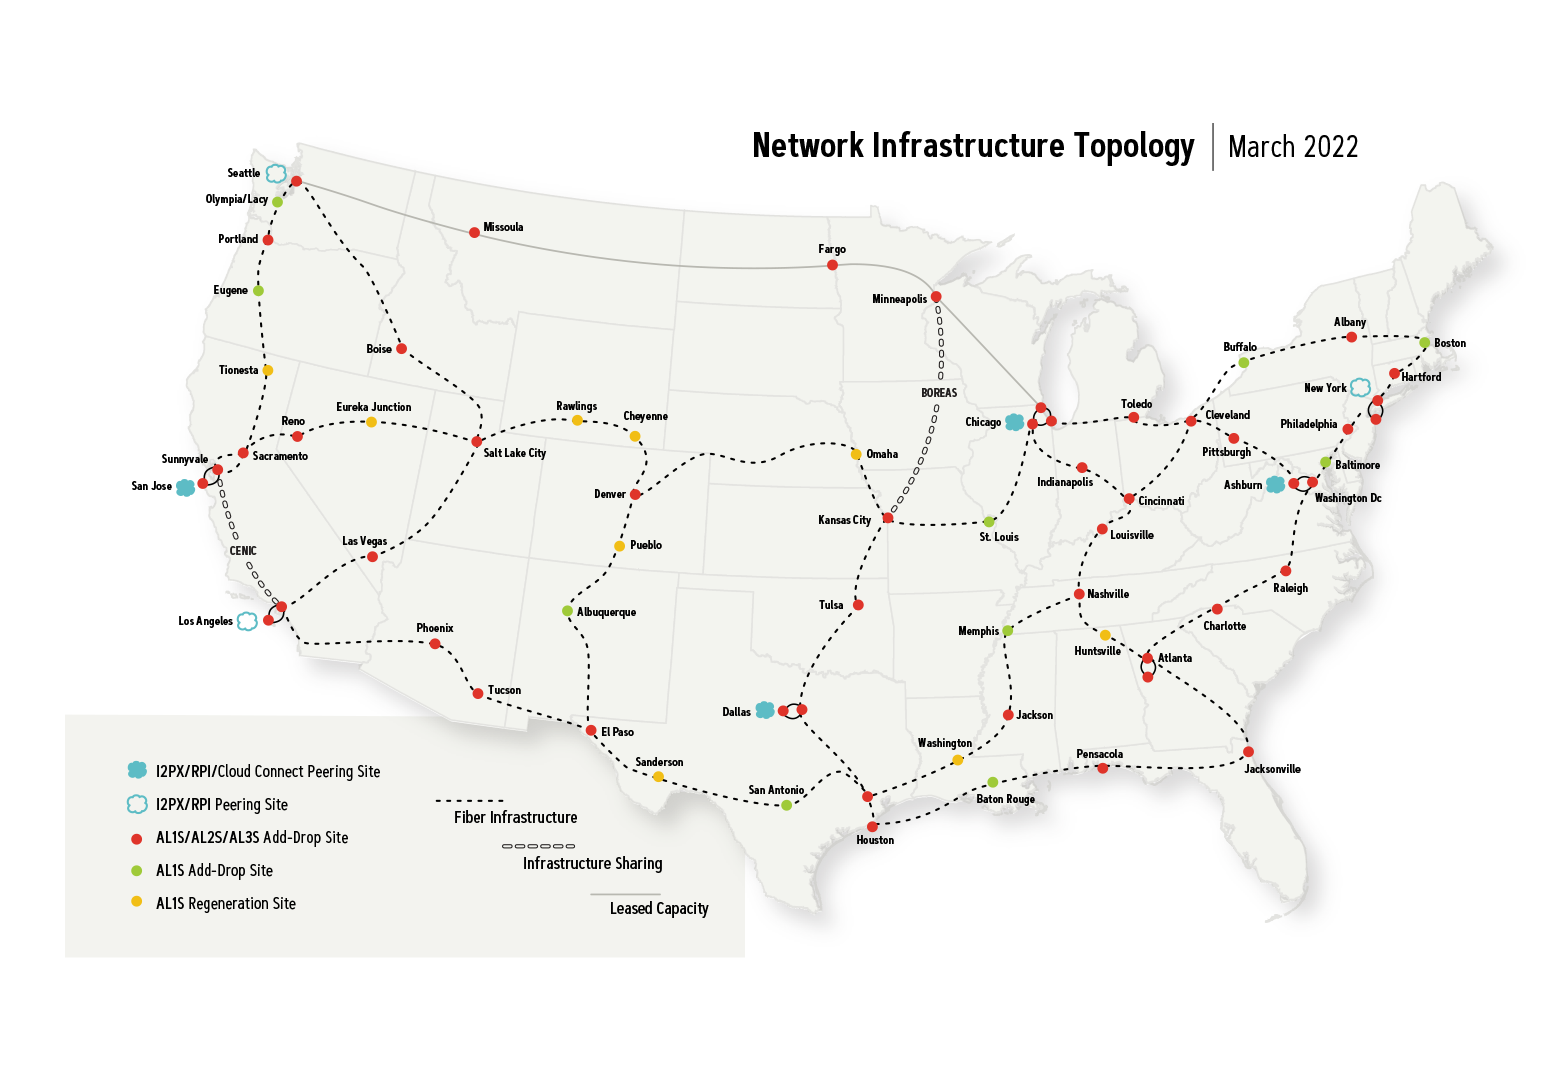
\includegraphics[width=\linewidth]{images/internet2.png}
        \end{adjustbox}
        % \caption{Caption for image 2}
        \label{fig:image2}
    \end{minipage}
\end{figure}


\end{block}

\end{column}

\separatorcolumn
\begin{column}{\colwidth}

\begin{block}{Identifying Hardware}
We sent unauthenticated Simple Network Management Protocol (SNMPv3) requests to routers. Some routers responded with an engine ID that contained a MAC address uniquely identifying the device. The first half of the MAC address identified the router vendor. We focused on finding patterns in the last 3 bytes of the MAC address to see if a network vendor might allocate specific devices to certain MAC addresses, but no such patterns emerged for routers in Internet2.

\begin{figure}[h]
    \centering
    \begin{adjustbox}{frame, bgcolor=black, center}
        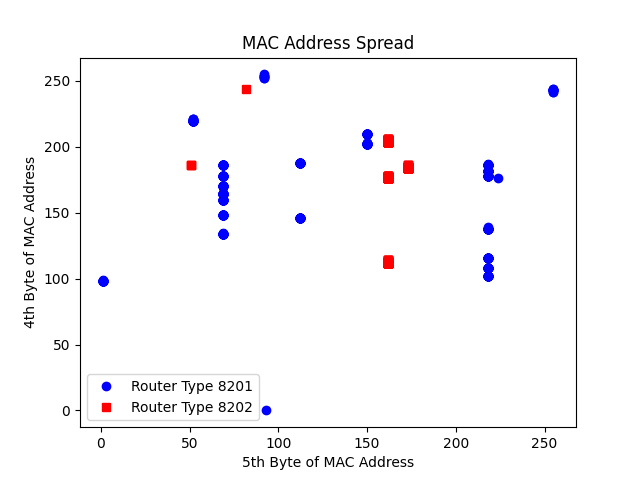
\includegraphics[width=0.7\textwidth]{images/mac_address.png}
    \end{adjustbox}
    % \caption{Image by OpenClipart-Vectors from Pixabay}
    \label{fig:figure2}
\end{figure}


\end{block}

\begin{block}{Computing Power Consumption}
We thoroughly examined publicly available information on each component involved in the routers used in Internet2 and NYSERnet and created a power calculator that breaks down the power consumption of individual hardware components. The power consumption varies based on load, power supply type, components used, and choice of optics deployed.
\

\begin{figure}[h]
    \centering
    \begin{minipage}{0.45\textwidth}
        \centering
        \begin{adjustbox}{frame, bgcolor=black, center}
            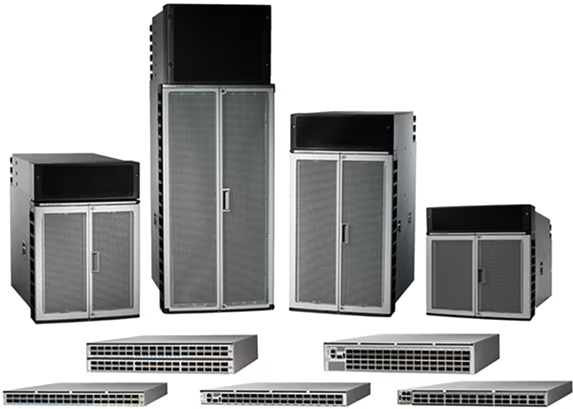
\includegraphics[width=\linewidth]{images/8000_routers.png}
        \end{adjustbox}
        % \caption{Caption for image 1}
        \label{fig:image1}
    \end{minipage}
    \hfill
    \begin{minipage}{0.5\textwidth}
        \centering
        \begin{adjustbox}{frame, bgcolor=black, center}
            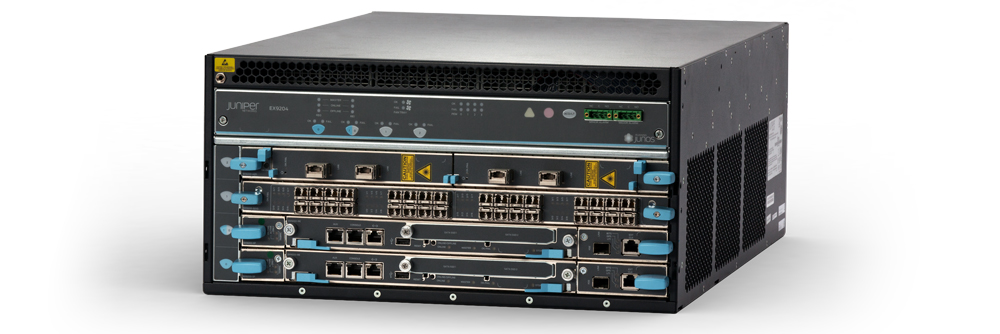
\includegraphics[width=\linewidth]{images/juniper_switch.png}
        \end{adjustbox}
        % \caption{Caption for image 2}
        \label{fig:image2}
    \end{minipage}
\end{figure}

\end{block}
\begin{block}{Conclusions}
Our research project showed that it is feasible to estimate the power consumption of ISPs in large-scale networks through alternative means of obtaining information. We found that the CAIDA dataset had extra routers and missing links, which may impact the accuracy of network topology analysis. Leveraging SNMPv3 provided valuable hardware information, but not all routers responded to requests. Our analysis of power consumption revealed that it varied based on several factors. Overall, our research provided insights into the practices of ISPs and highlighted potential areas for improvement in energy usage in large-scale networks.
\end{block}
\end{column}
\separatorcolumn

\end{columns}
\end{frame}

\end{document}
